\chapter{Introduction and theory}
\label{chap:theory}
In order to describe the search for invisible decays of the Higgs boson (``Higgs to invisible''), it is necessary to describe the theory behind them and also the statistical techniques used in carrying out the search. This chapter will start with an introduction to the current best theory of particle physics, the \ac{SM}, focussing on the Higgs mechanism, before outlining the motivations behind and some candidates for physics \ac{BSM}, then concluding with a discussion of the statistics of hypothesis testing. Natural units, where $\hbar=c=1$, Einstein summation convention and Feynman slash notation are used throughout. Four vector indices are labelled using greek letters, and gauge group generators using roman letters.

%??CHECK PLOT AXIS LABEL SIZES AND THAT LEGEND TERMS ARE STANDARD OR IN TEXT

\section{The standard model of particle physics}
\label{sec:SM}
The SM describes the interaction of the particles currently thought to be fundamental with the strong, weak and electromagnetic forces~\cite{GlashowPartialSymmetries,WeinbergModelOfLeptons,SalamNobelSymposium}. Its predictions, which come from specifying the symmetries the theory respects and how they are broken, the particles in the theory, and 18 free parameters, have been tested in many different experiments, in some cases up to one part in a trillion \cite{PhysRevLett.100.120801}. However, it does face challenges, described in section \SectionRef{sec:SMchallenges}, one example being that it does not describe \ac{DM}. 

The SM is a gauge invariant \ac{QFT}. To construct a QFT the symmetries that are respected by the theory and the fields it describes must be specified. The symmetries are important because of Noether's theorem, which states that for every continuously differentiable symmetry of the Lagrangian of a theory there is a corresponding conservation law~\cite{Noether:1918zz,doi:10.1080/00411457108231446}. An example of this is Poincar\'e invariance, the invariance of the laws of physics under translations and rotations in space and time, which leads through Noether's theorem to the conservation of energy, linear momentum and angular momentum. In addition to giving rise to conservation laws, some types of symmetry lead to additional fields being required to preserve invariance, this will be discussed further in \SectionRef{sec:gaugesym} \cite{PhysRev.96.191}.

It is important to specify the fields described by the QFT as these are constrained by the fundamental particles seen in nature. This is because particles correspond to the quantised excitations of fields. Specifically, scalar fields correspond to spin zero bosons, spinor fields correspond to spin half fermions, and vector fields correspond to spin 1 bosons. In order to add a new field an explanation for why the corresponding particle has not yet been observed must, therefore, be provided. We will now go through the particles observed in nature and how they are represented in the SM.

\subsection{Fundamental particles in nature}
There are two types of fundamental particles in nature, fermions and bosons. The fermions observed in nature that are currently thought to be fundamental are then divided into those which interact via the strong nuclear force (the quarks), and those which don't (the leptons). Both the quarks and leptons have two further types: charged and neutral in the case of the leptons, and up type and down type in the case of the fermions. Another interesting feature of the fermions is that they are arranged in three generations. Each generation has one fermion of each type with the same quantum numbers as those in the other generations, except that the mass is different. \TableRef{tab:fermions} shows this structure.

\begin{table}
  \caption{The fundamental fermions observed in nature separated into their three generations. Each particle shown also has an antiparticle with opposite charge and identical mass. Values taken from~\cite{Agashe:2014kda}}
  \label{tab:fermions}
  \begin{tabular}{ccccccc}
  \hhline{=======}
  &\multicolumn{3}{|c|}{Leptons}& \multicolumn{3}{c}{Hadrons} \\
  \cline{2-7}
  Generation & \multicolumn{1}{|c}{Particle} & Mass & \multicolumn{1}{c|}{Charge} & Particle & Mass & Charge \\
  \hhline{=======}
  \multirow{2}{*}{1} & \Pem & 511 \keV & -1 & \Pqu & 2.3 \MeV & $+\frac{2}{3}$ \\
  & \Pgne & $\sim$0 & 0 & \Pqd & 4.8 \MeV & $-\frac{1}{3}$ \\
  \hline
  \multirow{2}{*}{2} & \Pgmm & 105.7 \MeV & -1 & \Pqc & 1.275 \GeV & $+\frac{2}{3}$ \\
  & \Pgngm & $\sim$0 & 0 & \Pqs & 95 \MeV & $-\frac{1}{3}$ \\
  \hline
  \multirow{3}{*}{2} & \Pgtm & 1.777 \GeV & -1 & \Pqt & 173.2 \GeV & $+\frac{2}{3}$ \\
  & \Pgngt & $\sim$0 & 0 & \Pqb & 4.18 \GeV & $-\frac{1}{3}$ \\
  \hhline{=======}
  \end{tabular}
\end{table}

The bosons in nature also have two types. The first type are vector bosons which mediate the three fundamental interactions described by the SM. The vector bosons are summarised in \TableRef{tab:bosons}, where it can be seen that their masses are very different, the photon and the eight gluons being massless, while the \PWpm and \PZ bosons are very massive. As we will see in \SectionRef{sec:ssb} explaining these masses requires the Higgs mechanism. The Higgs mechanism also gives rise to the other type of boson seen in nature, the scalar Higgs boson. In order to see how all of the above particles are represented in the SM an introduction to gauge theories is necessary.

\begin{table}
  \caption{The fundamental vector bosons observed in nature separated by the force which they mediate. Values taken from~\cite{Agashe:2014kda}.}
  \label{tab:bosons}
  \begin{tabular}{lccc}
    \hline
    \hline
    Force & Particle & Mass & Charge \\
    \hhline{====}
    Electromagnetism & \Pgg & 0 & 0 \\
    \hline
    \multirow{2}{*}{Weak} & \PWpm & 80.4 \GeV & $\pm 1$ \\
    \cline{2-4}
    & \PZ & 91.2 \GeV & 0 \\
    \hline
    Strong & g & 0 & 0 \\
    \hline
    \hline
  \end{tabular}
\end{table}

\subsection{Introduction to gauge theories}
\label{sec:gaugesym}
Gauge symmetries are local transformations, i.e. the transformation can be different at different points in space and time, that form a symmetry group. To see the effect of imposing such a symmetry on a theory consider imposing local invariance under U(1) transformations on the Dirac Lagrangian for a masssive fermion:
\begin{equation}
  \label{eq:globaldiraclagrangian}
  \mathcal{L}=i\bar{\psi}\slashed{\partial}\psi-m\bar{\psi}\psi~\cite{griffiths2008introduction}.
\end{equation}

This Lagrangian is invariant under a global $U(1)$ transformation $\psi\rightarrow e^{iq\theta}\psi$, where q and $\theta$ are constant. However, if the $U(1)$ transformation is local i.e. $\theta$ is a function of spacetime position the Lagrangian is no longer invariant and transforms as:
\begin{equation}
  \label{eq:gaugeviolating}
  \mathcal{L}\rightarrow\mathcal{L}-q(\partial_{\mu}\theta)\bar{\psi}\gamma^{\mu}\psi.
\end{equation}

In order to restore invariance a vector field, $A_{\mu}$, referred to as a gauge field or gauge boson, which transforms as $A_{\mu}\rightarrow A_{\mu}+\partial_{\mu}\theta$ and has an interaction with the fermion field:
\begin{equation}
  \mathcal{L}_{int}=q(\bar{\psi}\gamma^{\mu}\psi) A_{\mu},
\end{equation}
 can be added to the theory. The interaction term of the new gauge field transforms as:
\begin{equation}
  \mathcal{L}_{int}\rightarrow \mathcal{L}_{int}+q(\partial_{\mu}\theta)\bar{\psi}\gamma^{\mu}\psi,
\end{equation}
which cancels out the non-gauge invariance seen in \EquationRef{eq:gaugeviolating}.

Assuming the new gauge field to be massless the Lagrangian is now:
\begin{equation}
  \label{eq:diraclag}
  \mathcal{L}=i\bar{\psi}\slashed{\partial}\psi-m\bar{\psi}\psi+q(\bar{\psi}\gamma^{\mu}\psi) A_{\mu}-\frac{1}{4}F_{\mu\nu}F^{\mu\nu},
\end{equation}
where $F_{\mu\nu}$ is the field strength tensor of the vector field. For a gauge boson from a general gauge group $F_{\mu\nu}$ is written as:
\begin{equation}
F_{\mu\nu}^a=\partial_{\mu}A_{\nu}^a-\partial_{\nu}A_{\mu}^a+gf&{abc}A_{\mu}^{b}A_{\nu}^{c},
\end{equation}
where $f^{abc}$ are the structure constants of the gauge group, which are a representation of the comutation relations between the group's generators. For $U(1)$ which only has one self-commuting generator the single structure constant is 0. However, for non-Abelian gauge groups (i.e. those with non-commuting generators) they can be non-zero causing the $F_{\mu\nu}F^{\mu\nu}$ term in the Lagrangian to include self-interaction terms of the vector bosons.

It is also interesting to note that \EquationRef{eq:diraclag} can be rewritten as:
\begin{equation}
  \label{eq:localdiraclagrangian}
  \mathcal{L}=i\bar{\psi}\gamma^{\mu}\mathcal{D}_{\mu}\psi-m\bar{\psi}\psi-\frac{1}{4}F_{\mu\nu}F^{\mu\nu},
\end{equation}
where $\mathcal{D}_{\mu}=\partial_{\mu}+iqA_{\mu}$ and is referred to as the covariant derivative. Comparing \EquationRef{eq:globaldiraclagrangian} and \EquationRef{eq:localdiraclagrangian} it can be seen that to go from a globally invariant Lagrangian to a locally invariant one we have substituted the normal spacetime derivative for the covariant derivative and added the free term of the vector field.

In the case of $U(1)$ transformations, which have one degree of freedom so can be described by one parameter, in the above case $\theta$, in order to make the Lagrangian locally invariant one interacting gauge boson had to be added. This correspondence between the number of degrees of freedom and the number of gauge bosons holds generally. For each degree of freedom of a group's transformations there exists a generator of the group, and for each generator one interacting gauge boson must be added to achieve local invariance.

%??give SM gauge group and fermion and vector representations 
\subsection{The SM gauge group and fundamental particle representations}
\label{sec:smgauge}
The SM is locally gauge invariant under the group $SU\left(3\right)_{C}\otimes SU\left(2\right)_{L}\otimes U\left(1\right)_{Y}$. Fermions in the SM are spin half spinor representations of these symmetry groups. These spinors can be split into chirally left and right handed components using the projection operators $P_{\substack{L \\R}}=\frac{1}{2}(1\mp \gamma^{5})$. Chirally left and right handed fermions transform differently under $SU\left(2\right)_{L}$. The right handed spinors are not charged under $SU\left(2\right)_{L}$ and thus are represented as a singlet, while the left handed spinors transform as a doublet.

The first generation of leptons can, therefore, be written as:
\begin{equation}
  \psi_{1}=\Pe_{R},\,\psi_{2}=L=\left(\begin{array}{c} \Pgne \\ \Pe_{L}\end{array}\right).
\end{equation}
The SM treats neutrinos as massless and has no right handed neutrino. Similarly the first generation of quarks can be written as:
\begin{equation}
  \psi_{3}=\Pqu_{R},\,\psi_{4}=\Pqd_{R},\,\psi_{5}=\left(\begin{array}{c} \Pqu_{L} \\ \Pqd_{L}\end{array}\right).
\end{equation}

As we saw in \SectionRef{sec:gaugesym} gauge symmetries in theories with fermions require the addition of an interacting vector boson per symmetry generator to preserve gauge invariance. $SU\left(3\right)_{C}$ has eight generators whose eight vector bosons, $G_{a\mu}$, correspond to the eight physical gluons of \ac{QCD}, which mediate the strong interaction. $SU\left(2\right)_{L}$ has three generators whose three vector bosons, $\PW^{i}_{\mu}$, mix with the one vector boson from $U\left(1\right)_{Y}$, $B_{\mu}$ unifying the electromagnetic and weak forces into one electroweak force. The physical states that result are:
\begin{equation}
  \begin{split}
  \PWpm_{\mu}=\frac{1}{\sqrt{2}}\left(\PW^{1}_{\mu}\mp i\PW^{2}_{\mu}\right) \\
  \PZ_{\mu}=cos\left(\theta_{W}\right)\PW^{3}_{\mu}-sin\left(\theta_{W}\right)B_{\mu} \\
  A_{\mu}=sin\left(\theta_{W}\right)\PW^{3}_{\mu}+cos\left(\theta_{W}\right)B_{\mu},
  \end{split}
\end{equation}
where $\theta_{W}$ is the Weinberg angle and $A_{\mu}$ is the photon field. Also, as described in \SectionRef{sec:gaugesym} the interaction between these vector bosons and the fermion fields occurs through their presence in the covariant derivative, and interactions between the vector bosons occur because $SU\left(3\right)_{C}$ and $SU\left(2\right)_{L}$ are non-Abelian.

Now let us try to construct a Lagrangian for these fields. First ignoring the masses we find:
\begin{equation}
  \mathcal{L}=i\bar{\psi}_{i}\slashed{\mathcal{D}}\psi_{i}-\frac{1}{4}F_{\mu\nu j}F^{\mu\nu}_{j},
\end{equation}
where the sum over all $\psi$ also includes the second and third generations, $F_{\mu\nu j}F^{\mu\nu}_{j}$ is a sum of the free terms of all the SM gauge bosons and $\mathcal{D}$ is the SM covariant derivative:
\begin{equation}
  \mathcal{D_{\mu}}=\partial_{\mu}+ig_{1}\frac{Y}{2}B_{\mu}+ig_{2}\frac{\tau_{i}}{2}W_{\mu}^{i}+ig_{3}\frac{\lambda_{a}}{2}G_{\mu}^{a},
\end{equation}
with Y being the constant generator of $U\left(1\right)$, $\tau_{i}$ the generators of $SU\left(2\right)_{L}$, $\lambda_{a}$ the generators of $SU\left(3\right)_{C}$ and $g_{i}$ the coupling constants of the fields. It should be noted that $\frac{g_{1}}{g_{2}}$ is equal to $\tan\left(\theta_{W}\right)$.

When we try to include mass a problem occurs. We know that some of the fermions have mass, and consequently we should have fermion mass terms of the form:
\begin{equation}
  \begin{split}
    \mathcal{L}_{m_{f}}&=-m_{f}\bar{f}{f} \\
    &=-m_{f}\bar{f}\left[\frac{1}{2}\left(1-\gamma^{5}\right)+\frac{1}{2}\left(1+\gamma^{5}\right)\right]f \\
    &=-m_{f}\left(\bar{f}_{R}f_{L}+\bar{f}_{L}f_{R}\right),
  \end{split}
\end{equation}
in our Lagrangian. However, as the left and right handed fields do not transform in the same way under $SU\left(2\right)_{L}$ this term breaks the gauge symmetry of the Lagrangian and can't be present. 

A similar problem occurs for vector fields. In \SectionRef{sec:gaugesym} we didn't consider the mass term of these vector fields:
\begin{equation}
  \label{eq:vectorlagrangian}
  \mathcal{L}_{m_V}=\frac{1}{2}m_{V}^{2}A_{\mu}A^{\mu},
\end{equation}
which is not gauge invariant, so it is not possible to include the massive vector bosons on their own in gauge invariant theories either. The additional piece of the SM required to allow particles to have mass is the Higgs mechanism.

\subsection{Spontaneous symmetry breaking and the Higgs mechanism}
\label{sec:ssb}
%??Introduce SSB
The Higgs mechanism is a form of spontaneous symmetry breaking~\cite{Englert:1964et,Higgs:1964ia,Higgs:1964pj,Guralnik:1964eu,Higgs:1966ev,Kibble:1967sv}. A symmetry is said to be spontaneously broken when the Lagrangian remains invariant while the vacuum state, i.e. that with lowest energy, does not~\cite{griffiths2008introduction}. Terms of the Lagrangian which are not gauge invariant can then be incorporated into the theory by adding a field which has a non-zero vacuum expectation value and coupling it to the other fields present in the term. For the Higgs mechanism this field is a complex scalar $SU\left(2\right)_{L}$ doublet, called the Higgs field:
\begin{equation}
\phi=\left(\begin{array}{c}\phi^+ \\ \phi^0 \end{array}\right).
\end{equation}
The main part of the Higgs field Lagrangian is:
\begin{equation}
  \label{eq:higlag}
\mathcal{L}=T-V=\left(\mathcal{D}_{\mu}\phi\right)^{\dag}\left(\mathcal{D}^{\mu}\phi\right)+\mu^{2}\phi^{\dag}\phi-\lambda\left(\phi^{\dag}\phi\right)^{2},
\end{equation}
Where the first two terms on the right hand side make up the kinetic part of the Higgs field Lagrangian, $T$, and the third term is the Higgs field potential, $V$. For $\mu^{2}>0$, the values of the Higgs field which minimise the Lagrangian are  non-zero and form a circle in phase space of $\phi$. All of these minima are equivalent and a particular minimum can be chosen with no physical effect. By convention we choose the following minimum:
\begin{equation}
  \bra{0}\phi\ket{0}=\left(\begin{array}{c} 0 \\ \sqrt{\frac{\mu^{2}}{2\lambda}} \end{array}\right)=\frac{1}{\sqrt{2}}\left(\begin{array}{c} 0 \\ v \end{array}\right).
\end{equation}
Next we consider small perturbations around this minimum. Ignoring perturbations that can be set to zero by gauge freedom gives:
\begin{equation}
  \phi=\left(\begin{array}{c}0 \\ v+H \end{array}\right).
\end{equation}
Inserting this into \EquationRef{eq:higlag} and ignoring terms with more than one type of field gives at leading order:
\begin{equation}
  \mathcal{L}=\frac{1}{2}\partial_{\mu}H\partial^{\mu}H-\frac{1}{2}\mu^{2}H^{2}+\frac{v^{2}}{8}\left[g_{2}^{2}W_{\mu}^{+}W^{+\mu}+g_{2}^{2}W_{\mu}^{-}W^{-\mu}+\left(g_{1}^{2}+g_{2}^{2}\right)Z_{\mu}Z^{\mu}\right].
\end{equation}
As expected, the weak vector bosons $W_{\mu}^{\pm}$ and $Z_{\mu}$ aquire masses $\frac{g_{2}v}{2}$ and $\frac{v}{2}\sqrt{g_{1}^{2}+g_{1}^{2}}$ respectively. We also see an additional massive scalar $H$, which is the Higgs boson, which has mass $\sqrt{2}\mu$. The photon and gluons do not aquire masses as the particular choice of coupling constants and the structure of the group generators leads to the terms in $A_{\mu}$ and $G_{\mu a}$ being zero.

The final part of the Higgs field Lagrangian is that giving rise to the fermion masses. These are generated by a Yukawa term in the Lagrangian for each fermion as follows:
\begin{equation}
  \mathcal{L}_{Yuk}=k_{f}\left(\bar{f}_{L}\phi f_{R}+\bar{f}_{R}\phi^{\dag}f_{L}\right),
\end{equation}
where $k_{f}$ is the Yukawa coupling. The fermion's mass is then $\frac{k_{f}v}{\sqrt{2}}$, so heavier fermions couple more strongly to the Higgs boson. The \ac{SM} provides no prediction of, or relationship between, the Yukawa couplings of the fermions, however they can be determined using the observed masses of the fermions.

%??note about which of the above params are known/predicted and which are free and how this leaves room for BSM and ref


\subsection{Challenges for the SM}
\label{sec:SMchallenges}


\section{Dark matter}
\label{sec:DM}
%??Introduce dark matter and motivate search for it and other invisible final states in Higgs decays

\subsection{Searching for dark matter with Higgs bosons}
\label{sec:higgsdm}
%??mention collider searches for Dark matter use MET and need associated production
%??Introduce jets and MET
%??CMS in full


\subsection{Some extensions of the standard model incorporating dark matter}
\label{sec:DMextensions}
%??Introduce theories that are used for pheno work


\section{Higgs boson production and decay at the LHC}
\label{sec:higprod}
%??Detail Higgs production and decays in order to motivate searching for invisible decays in the VBF channel
The Large Hadron Collider (\LHC) (discussed in detail in \SectionRef{sec:lhc}) collides protons at high energies. The results of these collisions are referred to as ``events''. The dominant production mechanisms for Higgs bosons in high energy proton collisions are shown in \FigureRef{fig:smprodfeyn}, and they have the cross-sections shown in \FigureRef{fig:smprodfeyn}. It can be seen that \ac{ggH} production, where two gluons fuse via a quark loop to produce a Higgs boson (as shown in \FigureRef{fig:smprodfeyn}a), has the highest cross-section across the full Higgs boson mass range shown. Unfortunately, this production mode normally results in no visible particles in the final state and therefore most \ac{ggH} events cannot be used to search for invisibly decaying Higgs boson. In some \ac{ggH} events there is \ac{QCD} radiation from the initial state particles (\ac{ISR}), which can result in visible jets in the final state and thus allow invisibly decaying Higgs boson searches to be performed. However, the visible particles in these events are hard to distinguish from other similar \ac{QCD} background processes with much larger cross-sections, so \ac{ggH} is not the most promising channel for invisibly decaying Higgs boson searches.

The next highest cross-section production process is \ac{VBF}. As can be seen in \FigureRef{fig:smprodfeyn}b, this process involves two incoming quarks both radiating vector bosons which then fuse resulting in a Higgs boson. The two initial quarks form jets in the final state, providing visible particles with which to perform an invisibly decaying Higgs boson search. Furthermore, the lack of a strong force connection (referred to as ``colour connection'') between the two quarks means that the resulting jets have a distinctive topology, being well separated and also that there is very little other hadronic activity in \ac{VBF} events. This distinctive topology and high cross-section make \ac{VBF} the most sensitive production channel for invisibly decaying Higgs boson searches. For this reason, this thesis will focus on the \ac{VBF} channel.

After \ac{VBF}, \ac{VH} production has the next highest cross-section. \ac{VH} production results in a Higgs boson and a vector boson, which decays resulting in visible particles in the final state allowing invisibly decaying Higgs boson searches to be carried out. In the case of leptonic vector boson decays, these final state particles can be relatively easy to identify resulting in lower backgrounds than in the case of searches in the \ac{VBF} and \ac{ggH} channels. However, the lower cross-section means that the \ac{VH} channel is not as sensitive as \ac{VBF}.

Finally, the fourth highest cross-section Higgs boson production channel is top quark associated production, where the final state consists of two top quarks and a Higgs boson. Whilst, the top quarks do decay to visible particles which could be identified, the cross-section for this process is too low, and the backgrounds are too high for an invisibly decaying Higgs boson search to be carried out using the Run 1 \LHC data.

\begin{figure}
    %ggh
  \subfloat[]{
    \begin{fmfgraph*}(150,150)
      \fmfleft{i0,i2,ix,i3,i5}
      \fmfright{o0,o3,o1,o4,o6}
      \fmf{phantom,tension=4/3}{i2,v1,o3}
      \fmf{phantom,tension=4/3}{i3,v2,o4}
      \fmffreeze
      \fmf{gluon,tension=4/3}{i2,v1}
      \fmf{gluon,tension=4/3}{i3,v2}
      \fmf{fermion,tension=0}{v1,v2}
      \fmf{fermion,tension=2/3}{v2,v3,v1}
      \fmf{dashes}{v3,o1}
      \fmflabel{$g$}{i2}
      \fmflabel{$g$}{i3}
      \fmflabel{$H$}{o1}
  \end{fmfgraph*}}    
  %vbf
  \hspace{3.5cm}
  \subfloat[]{
    \begin{fmfgraph*}(150,150)
      \fmfleft{i1,i2}
      \fmfright{o1,o2,o3}
      \fmf{fermion}{i1,v1,o1}
      \fmf{fermion}{i2,v2,o3}
      \fmf{photon,label=$W,,Z$}{v1,v3}
      \fmf{photon,label=$W,,Z$}{v2,v3}
      \fmf{dashes}{v3,o2}
      \fmflabel{$q$}{i1}
      \fmflabel{$q$}{i2}
      \fmflabel{$q$}{o1}
      \fmflabel{$q$}{o3}
      \fmflabel{$H$}{o2}
  \end{fmfgraph*}
  \vspace{.5cm}
}

  \vspace{.5cm}
  
    %Higgstrahlung
  \subfloat[]{
    \begin{fmfgraph*}(150,150)
      \fmfleft{i1,i2}
      \fmfright{o1,o2}
      \fmf{fermion}{i1,v1}
      \fmf{fermion}{v1,i2}
      \fmf{photon,label=$W,,Z$}{v1,v2}
      \fmf{photon}{v2,o1}
      \fmf{dashes}{v2,o2}
      \fmflabel{$q$}{i1}
      \fmflabel{$\bar{q}$}{i2}
      \fmflabel{$W,Z$}{o1}
      \fmflabel{$H$}{o2}
  \end{fmfgraph*}
  \vspace{.5cm}
}
  \hspace{3.5cm}
  %tth
  \subfloat[]{
    \begin{fmfgraph*}(150,150)
      \fmfleft{i0,i1,i4,i5,i6,i2,i3}
      \fmfright{o0,o1,o2,o3,o4}
      \fmf{gluon,tension=3/2}{i1,v1}
      \fmf{gluon,tension=3/2}{i2,v2}
      \fmf{fermion}{o1,v1,v3,v2,o3}
      \fmf{dashes,tension=3/2}{v3,o2}
      \fmflabel{$g$}{i1}
      \fmflabel{$g$}{i2}
      \fmflabel{$\bar{t}$}{o1}
      \fmflabel{$t$}{o3}
      \fmflabel{$H$}{o2}
  \end{fmfgraph*}
}
  
  \caption{Feynman diagrams for the four \ac{SM} Higgs boson production processes with the highest cross-sections: \ac{ggH} (a), \ac{VBF} (b), \ac{VH} (c) and top quark associated production (d).}
  \label{fig:smprodfeyn}
\end{figure}

\begin{figure}
  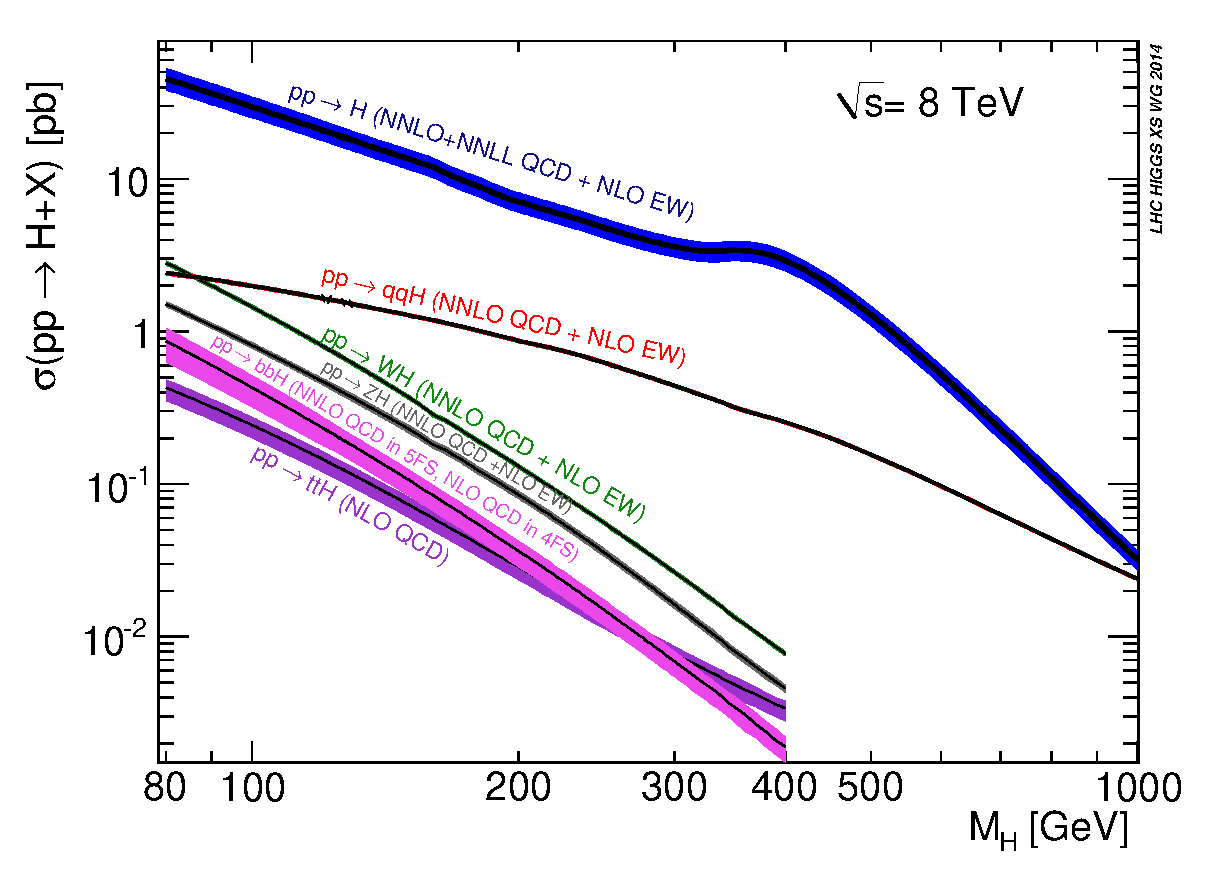
\includegraphics[width=\largefigwidth]{plots/theory/XS_8TeV.eps}
  \caption{Cross-sections for Higgs boson production via the most common production processes at $\sqrt{s}=8 \TeV$ as a function of Higgs boson mass, $m_{H}$~\cite{Heinemeyer:1559921}. The widths of the lines represent the theoretical uncertainties on the cross-section calculation.}
  \label{fig:smprod}
\end{figure}

%??talk about SM decays and what SM invisible branching fraction is, direct vs indirect
As mentioned in \SectionRef{sec:higgsdm} limits can be placed on the Higgs boson's coupling to \ac{DM} by %??explain indirect
%??Mention BRINV


\begin{figure}
  \subfloat{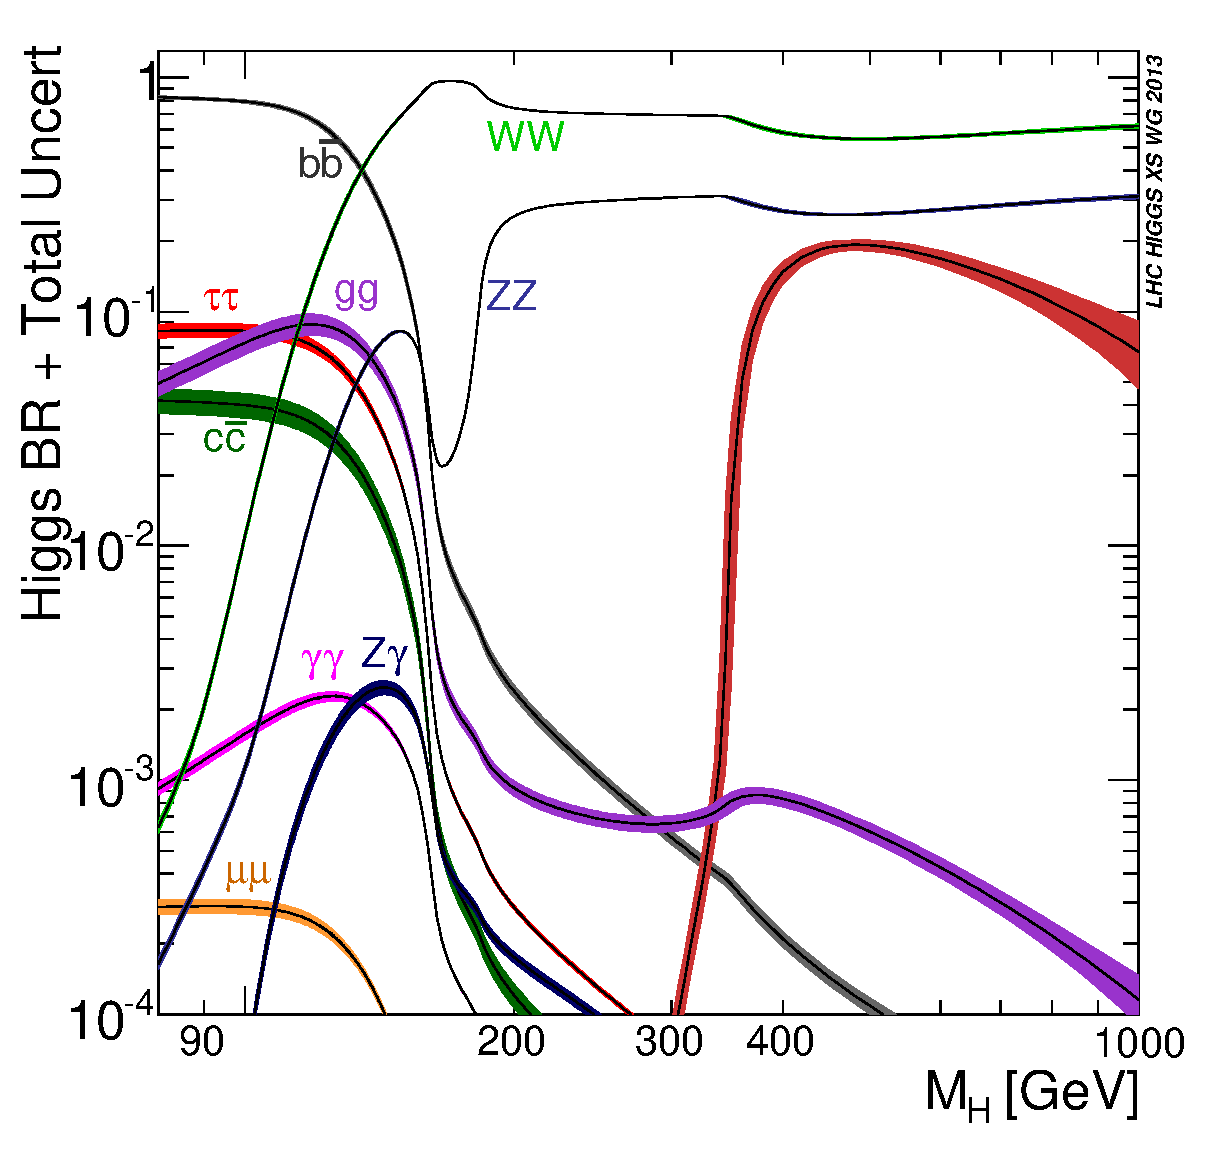
\includegraphics[width=.65\largefigwidth]{plots/theory/Higgs_BR.eps}}
  \subfloat{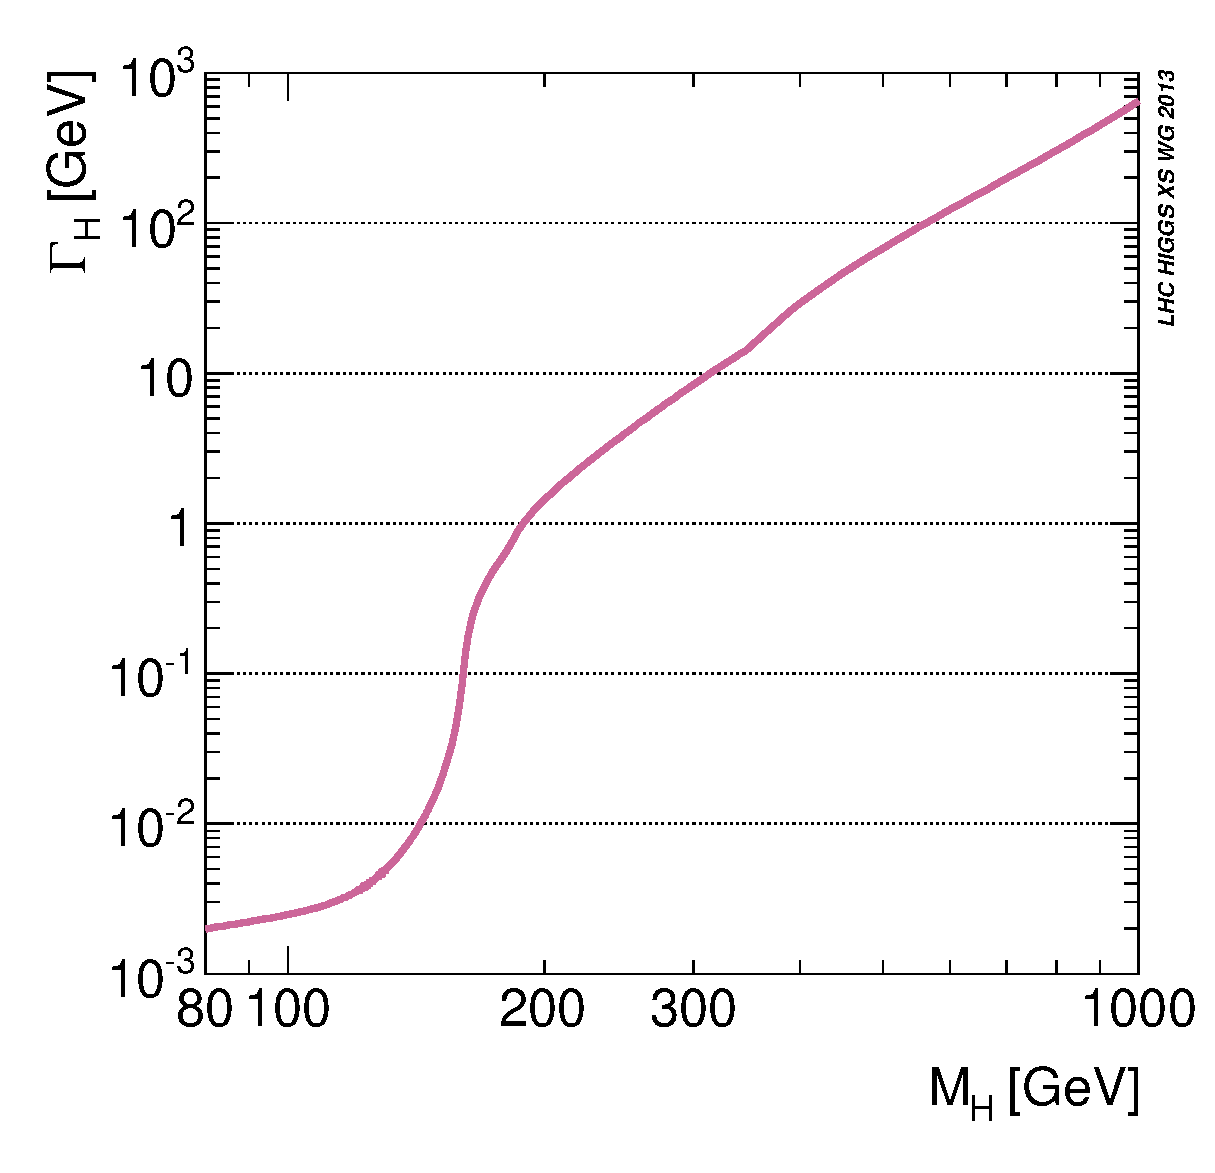
\includegraphics[width=.65\largefigwidth]{plots/theory/SM_Width.eps}}

  \caption{Branching ratios for the dominant Higgs boson decays as a function of Higgs boson mass with the line widths representing the uncertainties (a), and the \ac{SM} Higgs boson total width, $\Gamma_{H}$, as a function of Higgs boson mass (b)~\cite{Heinemeyer:1559921}.}
  \label{fig:smdecay}
\end{figure}


%??Mention proportionality of higgs coupling and mass

\section{Simulation}
\label{sec:sim}
%??introduce simulation
%??pdf and qcd scale
%??different generators including MCFM, VBFNLO, FEWZ, pythia, powheg, madgraph
%??explain generator level, parton level
%??weights: W soup, pileup, lepton weights, cross-section, top reweighting
\label{sec:mcweights}
%??output of four vectors of particles

\section{Statistics of exclusion limits}
\label{sec:stats}
%??introduce cls and limit setting
Limits on the parameters of theoretical models are presented throughout this thesis. The limits are set by performing a hypothesis test to discriminate between a null, background physics model only, hypothesis, $b$ and a test hypothesis, the signal process, $s$, plus background model. The particular procedure used is based on the CL$_{S}$ statistic and was developed by the LHC Higgs Combination Group and is used by both the ATLAS and CMS experiments~\cite{ATL-PHYS-PUB-2011-011}. 

The procedure starts by defining a likelihood function, $\mathcal{L}$, which quantifies how likely a given observation is given the expectation under a given hypothesis. $\mathcal{L}$ takes the form:
\begin{equation}
  \label{eq:likelihood}
  \mathcal{L}=\displaystyle\prod_{i}Poisson\left(n_{i}|\nu_{i}\left(\mu,\theta\right)\right)\cdot\prod_{j}Constraint\left(\theta_{j},\bar{\theta}\right),
\end{equation}
where the first term is the contribution from the Poisson probability to observe $n_{i}$ events in each analysis category, $i$, considered given a predicted number of events from the hypothesis, $\nu_{i}$. $\nu_{i}$ is a function of a signal strength parameter, $\mu$, which in the case of the signal hypothesis being an SM Higgs boson is 1 for the SM and 0 for the background only case, and the ``nuisance paramters,'' $\theta$, which account for the uncertainties on parameters of the signal and background models and any correlations between them. The second term in \EquationRef{eq:likelihood} represents the constraints on the allowed values of these nuisance parameters, with $\bar{\theta}$ being the best estimate of $\theta$ obtained from external measurements. The shape of the constraint function varies depending on the nuisance parameter it represents. For example, uncertainties on the event yield in a category are usually modelled with log-normal constraints, which exclude negative values of the event yield. 

Profile likelihood ratios, q$_{\mu}$, are then calculated, which are defined as:
\begin{equation}
  \label{eq:proflikelihood}
  q_{\mu} = -2 \ln\frac{\mathcal{L}(obs|\mu \cdot s + b,\hat{\theta}_{\mu})}{\mathcal{L}(obs|\hat{\mu} \cdot s + b,\hat{\theta})}\,,
\end{equation}
where $obs$ is the observation, and $\hat{\mu}$ and $\hat{\theta}$ are the values of $\theta$ and the $\mu$ where the likelihood is maximised given the constraint $0 \geqslant \hat{\mu} \geqslant \mu$. $\hat{\theta}_{\mu}$ are the values of the nuisance parameters that maximise the likelihood for a given $\mu$. The profile likelihood ratio therefore describes how likely it is to observe a signal strength equal to or higher than $\mu$ compared to the most likely signal strength.

Finally the CL$_{s}$ statistic itself is defined as:
\begin{equation}
  \label{eq:cls}
  CL_{s} = \frac{P(q_{\mu}\geqslant q_{\mu}^{obs} | \mu \cdot s + b)}{P(q_{\mu}\geqslant q_{\mu}^{obs}|b)}\,,
\end{equation}
Where the probability $P$ of a given $q_{\mu}$ is calculated using the asymptotic limit approximation~\cite{Cowan:2010js}. The region in which a signal strength $\mu \cdot s$ is excluded with $1 - \alpha$ \ac{CL} is then the region for which CL$_{s}$ is less than or equal to $\alpha$, i.e. when the signal hypothesis is $\alpha$ times less probably than the background.
